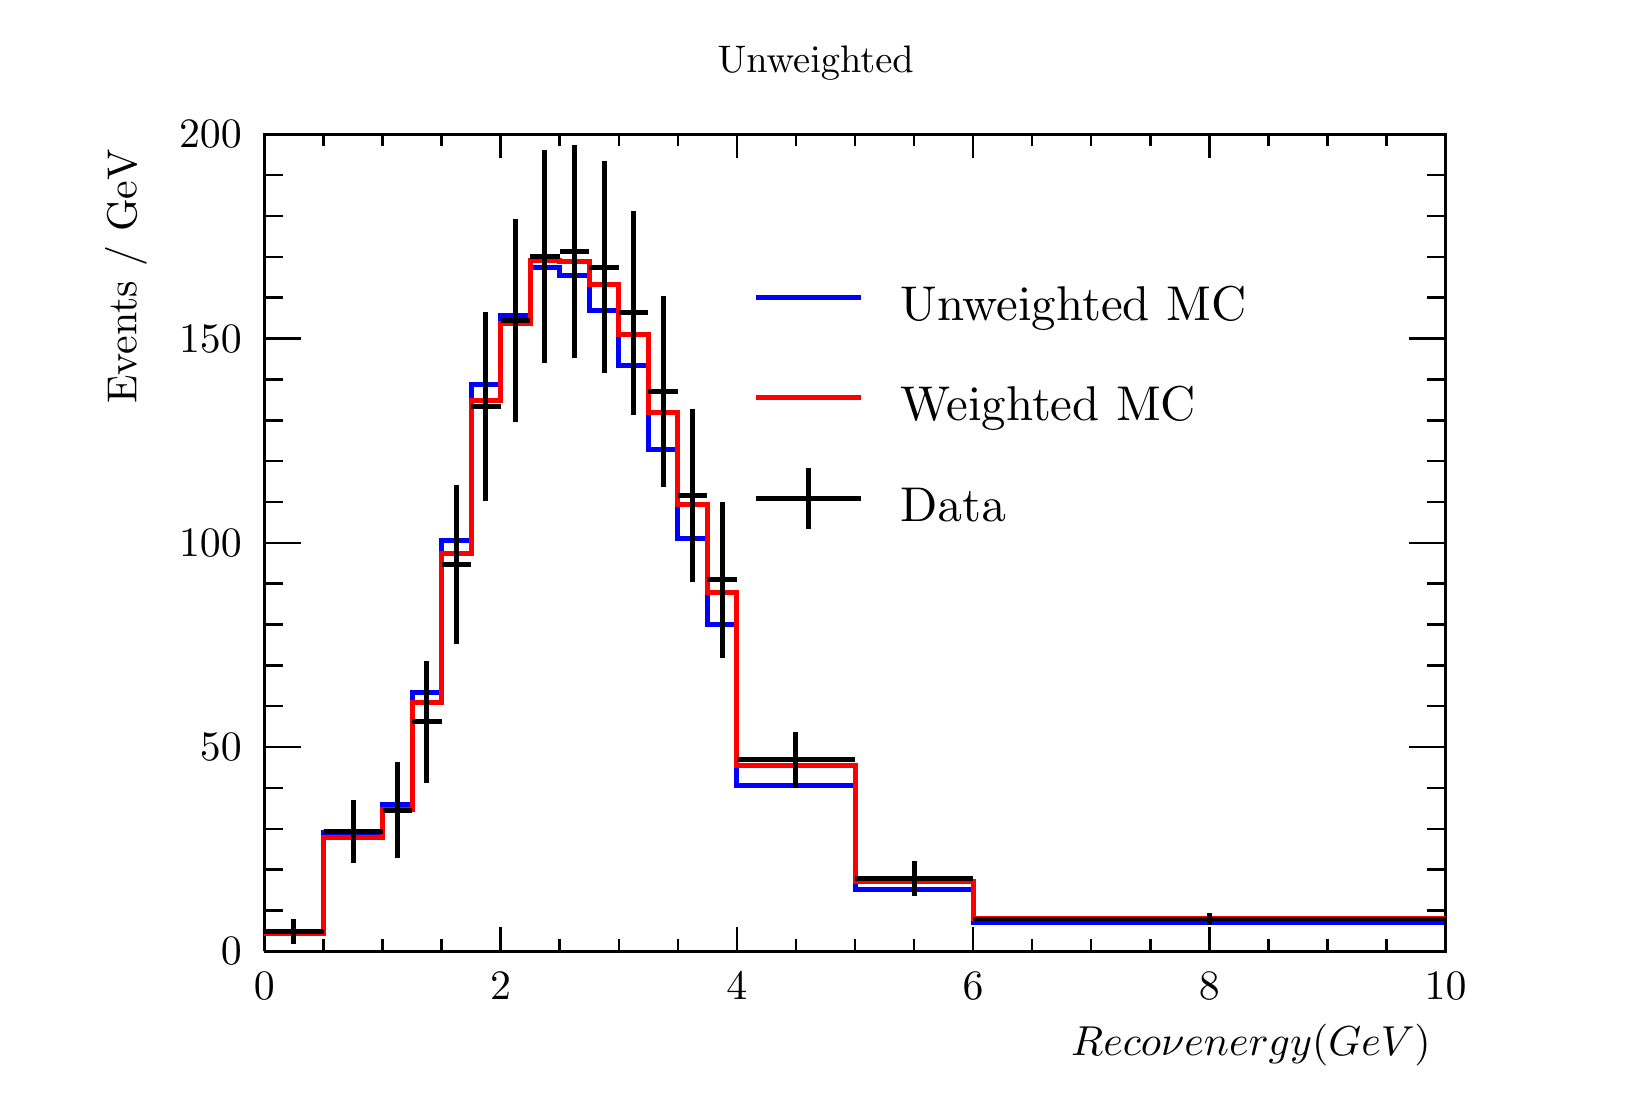
\begin{tikzpicture}
\pgfdeclareplotmark{cross} {
\pgfpathmoveto{\pgfpoint{-0.3\pgfplotmarksize}{\pgfplotmarksize}}
\pgfpathlineto{\pgfpoint{+0.3\pgfplotmarksize}{\pgfplotmarksize}}
\pgfpathlineto{\pgfpoint{+0.3\pgfplotmarksize}{0.3\pgfplotmarksize}}
\pgfpathlineto{\pgfpoint{+1\pgfplotmarksize}{0.3\pgfplotmarksize}}
\pgfpathlineto{\pgfpoint{+1\pgfplotmarksize}{-0.3\pgfplotmarksize}}
\pgfpathlineto{\pgfpoint{+0.3\pgfplotmarksize}{-0.3\pgfplotmarksize}}
\pgfpathlineto{\pgfpoint{+0.3\pgfplotmarksize}{-1.\pgfplotmarksize}}
\pgfpathlineto{\pgfpoint{-0.3\pgfplotmarksize}{-1.\pgfplotmarksize}}
\pgfpathlineto{\pgfpoint{-0.3\pgfplotmarksize}{-0.3\pgfplotmarksize}}
\pgfpathlineto{\pgfpoint{-1.\pgfplotmarksize}{-0.3\pgfplotmarksize}}
\pgfpathlineto{\pgfpoint{-1.\pgfplotmarksize}{0.3\pgfplotmarksize}}
\pgfpathlineto{\pgfpoint{-0.3\pgfplotmarksize}{0.3\pgfplotmarksize}}
\pgfpathclose
\pgfusepathqstroke
}
\pgfdeclareplotmark{cross*} {
\pgfpathmoveto{\pgfpoint{-0.3\pgfplotmarksize}{\pgfplotmarksize}}
\pgfpathlineto{\pgfpoint{+0.3\pgfplotmarksize}{\pgfplotmarksize}}
\pgfpathlineto{\pgfpoint{+0.3\pgfplotmarksize}{0.3\pgfplotmarksize}}
\pgfpathlineto{\pgfpoint{+1\pgfplotmarksize}{0.3\pgfplotmarksize}}
\pgfpathlineto{\pgfpoint{+1\pgfplotmarksize}{-0.3\pgfplotmarksize}}
\pgfpathlineto{\pgfpoint{+0.3\pgfplotmarksize}{-0.3\pgfplotmarksize}}
\pgfpathlineto{\pgfpoint{+0.3\pgfplotmarksize}{-1.\pgfplotmarksize}}
\pgfpathlineto{\pgfpoint{-0.3\pgfplotmarksize}{-1.\pgfplotmarksize}}
\pgfpathlineto{\pgfpoint{-0.3\pgfplotmarksize}{-0.3\pgfplotmarksize}}
\pgfpathlineto{\pgfpoint{-1.\pgfplotmarksize}{-0.3\pgfplotmarksize}}
\pgfpathlineto{\pgfpoint{-1.\pgfplotmarksize}{0.3\pgfplotmarksize}}
\pgfpathlineto{\pgfpoint{-0.3\pgfplotmarksize}{0.3\pgfplotmarksize}}
\pgfpathclose
\pgfusepathqfillstroke
}
\pgfdeclareplotmark{newstar} {
\pgfpathmoveto{\pgfqpoint{0pt}{\pgfplotmarksize}}
\pgfpathlineto{\pgfqpointpolar{44}{0.5\pgfplotmarksize}}
\pgfpathlineto{\pgfqpointpolar{18}{\pgfplotmarksize}}
\pgfpathlineto{\pgfqpointpolar{-20}{0.5\pgfplotmarksize}}
\pgfpathlineto{\pgfqpointpolar{-54}{\pgfplotmarksize}}
\pgfpathlineto{\pgfqpointpolar{-90}{0.5\pgfplotmarksize}}
\pgfpathlineto{\pgfqpointpolar{234}{\pgfplotmarksize}}
\pgfpathlineto{\pgfqpointpolar{198}{0.5\pgfplotmarksize}}
\pgfpathlineto{\pgfqpointpolar{162}{\pgfplotmarksize}}
\pgfpathlineto{\pgfqpointpolar{134}{0.5\pgfplotmarksize}}
\pgfpathclose
\pgfusepathqstroke
}
\pgfdeclareplotmark{newstar*} {
\pgfpathmoveto{\pgfqpoint{0pt}{\pgfplotmarksize}}
\pgfpathlineto{\pgfqpointpolar{44}{0.5\pgfplotmarksize}}
\pgfpathlineto{\pgfqpointpolar{18}{\pgfplotmarksize}}
\pgfpathlineto{\pgfqpointpolar{-20}{0.5\pgfplotmarksize}}
\pgfpathlineto{\pgfqpointpolar{-54}{\pgfplotmarksize}}
\pgfpathlineto{\pgfqpointpolar{-90}{0.5\pgfplotmarksize}}
\pgfpathlineto{\pgfqpointpolar{234}{\pgfplotmarksize}}
\pgfpathlineto{\pgfqpointpolar{198}{0.5\pgfplotmarksize}}
\pgfpathlineto{\pgfqpointpolar{162}{\pgfplotmarksize}}
\pgfpathlineto{\pgfqpointpolar{134}{0.5\pgfplotmarksize}}
\pgfpathclose
\pgfusepathqfillstroke
}
\definecolor{c}{rgb}{1,1,1};
\draw [color=c, fill=c] (0,0) rectangle (20,13.4752);
\draw [color=c, fill=c] (3,1.75177) rectangle (18,12.1277);
\definecolor{c}{rgb}{0,0,0};
\draw [c,line width=0.9] (3,1.75177) -- (3,12.1277) -- (18,12.1277) -- (18,1.75177) -- (3,1.75177);
\definecolor{c}{rgb}{1,1,1};
\draw [color=c, fill=c] (3,1.75177) rectangle (18,12.1277);
\definecolor{c}{rgb}{0,0,0};
\draw [c,line width=0.9] (3,1.75177) -- (3,12.1277) -- (18,12.1277) -- (18,1.75177) -- (3,1.75177);
\definecolor{c}{rgb}{0,0,1};
\draw [c,line width=1.8] (3,1.98647) -- (3.75,1.98647) -- (3.75,3.25573) -- (4.5,3.25573) -- (4.5,3.6191) -- (4.875,3.6191) -- (4.875,5.04048) -- (5.25,5.04048) -- (5.25,6.97323) -- (5.625,6.97323) -- (5.625,8.94826) -- (6,8.94826) -- (6,9.82879) --
 (6.375,9.82879) -- (6.375,10.4386) -- (6.75,10.4386) -- (6.75,10.3354) -- (7.125,10.3354) -- (7.125,9.89162) -- (7.5,9.89162) -- (7.5,9.19114) -- (7.875,9.19114) -- (7.875,8.12045) -- (8.25,8.12045) -- (8.25,6.99477) -- (8.625,6.99477) --
 (8.625,5.90293) -- (9,5.90293) -- (9,3.85844) -- (10.5,3.85844) -- (10.5,2.54063) -- (12,2.54063) -- (12,2.12032) -- (18,2.12032);
\definecolor{c}{rgb}{0,0,0};
\draw [c,line width=0.9] (3,1.75177) -- (18,1.75177);
\draw [c,line width=0.9] (3,2.05496) -- (3,1.75177);
\draw [c,line width=0.9] (3.75,1.90337) -- (3.75,1.75177);
\draw [c,line width=0.9] (4.5,1.90337) -- (4.5,1.75177);
\draw [c,line width=0.9] (5.25,1.90337) -- (5.25,1.75177);
\draw [c,line width=0.9] (6,2.05496) -- (6,1.75177);
\draw [c,line width=0.9] (6.75,1.90337) -- (6.75,1.75177);
\draw [c,line width=0.9] (7.5,1.90337) -- (7.5,1.75177);
\draw [c,line width=0.9] (8.25,1.90337) -- (8.25,1.75177);
\draw [c,line width=0.9] (9,2.05496) -- (9,1.75177);
\draw [c,line width=0.9] (9.75,1.90337) -- (9.75,1.75177);
\draw [c,line width=0.9] (10.5,1.90337) -- (10.5,1.75177);
\draw [c,line width=0.9] (11.25,1.90337) -- (11.25,1.75177);
\draw [c,line width=0.9] (12,2.05496) -- (12,1.75177);
\draw [c,line width=0.9] (12.75,1.90337) -- (12.75,1.75177);
\draw [c,line width=0.9] (13.5,1.90337) -- (13.5,1.75177);
\draw [c,line width=0.9] (14.25,1.90337) -- (14.25,1.75177);
\draw [c,line width=0.9] (15,2.05496) -- (15,1.75177);
\draw [c,line width=0.9] (15.75,1.90337) -- (15.75,1.75177);
\draw [c,line width=0.9] (16.5,1.90337) -- (16.5,1.75177);
\draw [c,line width=0.9] (17.25,1.90337) -- (17.25,1.75177);
\draw [c,line width=0.9] (18,2.05496) -- (18,1.75177);
\draw [anchor=base] (3,1.14539) node[scale=1.51215, color=c, rotate=0]{0};
\draw [anchor=base] (6,1.14539) node[scale=1.51215, color=c, rotate=0]{2};
\draw [anchor=base] (9,1.14539) node[scale=1.51215, color=c, rotate=0]{4};
\draw [anchor=base] (12,1.14539) node[scale=1.51215, color=c, rotate=0]{6};
\draw [anchor=base] (15,1.14539) node[scale=1.51215, color=c, rotate=0]{8};
\draw [anchor=base] (18,1.14539) node[scale=1.51215, color=c, rotate=0]{10};
\draw [anchor= east] (18,0.565957) node[scale=1.51215, color=c, rotate=0]{$Reco \nu energy (GeV)$};
\draw [c,line width=0.9] (3,12.1277) -- (18,12.1277);
\draw [c,line width=0.9] (3,11.8245) -- (3,12.1277);
\draw [c,line width=0.9] (3.75,11.9761) -- (3.75,12.1277);
\draw [c,line width=0.9] (4.5,11.9761) -- (4.5,12.1277);
\draw [c,line width=0.9] (5.25,11.9761) -- (5.25,12.1277);
\draw [c,line width=0.9] (6,11.8245) -- (6,12.1277);
\draw [c,line width=0.9] (6.75,11.9761) -- (6.75,12.1277);
\draw [c,line width=0.9] (7.5,11.9761) -- (7.5,12.1277);
\draw [c,line width=0.9] (8.25,11.9761) -- (8.25,12.1277);
\draw [c,line width=0.9] (9,11.8245) -- (9,12.1277);
\draw [c,line width=0.9] (9.75,11.9761) -- (9.75,12.1277);
\draw [c,line width=0.9] (10.5,11.9761) -- (10.5,12.1277);
\draw [c,line width=0.9] (11.25,11.9761) -- (11.25,12.1277);
\draw [c,line width=0.9] (12,11.8245) -- (12,12.1277);
\draw [c,line width=0.9] (12.75,11.9761) -- (12.75,12.1277);
\draw [c,line width=0.9] (13.5,11.9761) -- (13.5,12.1277);
\draw [c,line width=0.9] (14.25,11.9761) -- (14.25,12.1277);
\draw [c,line width=0.9] (15,11.8245) -- (15,12.1277);
\draw [c,line width=0.9] (15.75,11.9761) -- (15.75,12.1277);
\draw [c,line width=0.9] (16.5,11.9761) -- (16.5,12.1277);
\draw [c,line width=0.9] (17.25,11.9761) -- (17.25,12.1277);
\draw [c,line width=0.9] (18,11.8245) -- (18,12.1277);
\draw [c,line width=0.9] (3,1.75177) -- (3,12.1277);
\draw [c,line width=0.9] (3.462,1.75177) -- (3,1.75177);
\draw [c,line width=0.9] (3.231,2.27057) -- (3,2.27057);
\draw [c,line width=0.9] (3.231,2.78936) -- (3,2.78936);
\draw [c,line width=0.9] (3.231,3.30816) -- (3,3.30816);
\draw [c,line width=0.9] (3.231,3.82695) -- (3,3.82695);
\draw [c,line width=0.9] (3.462,4.34574) -- (3,4.34574);
\draw [c,line width=0.9] (3.231,4.86454) -- (3,4.86454);
\draw [c,line width=0.9] (3.231,5.38333) -- (3,5.38333);
\draw [c,line width=0.9] (3.231,5.90213) -- (3,5.90213);
\draw [c,line width=0.9] (3.231,6.42092) -- (3,6.42092);
\draw [c,line width=0.9] (3.462,6.93972) -- (3,6.93972);
\draw [c,line width=0.9] (3.231,7.45851) -- (3,7.45851);
\draw [c,line width=0.9] (3.231,7.97731) -- (3,7.97731);
\draw [c,line width=0.9] (3.231,8.4961) -- (3,8.4961);
\draw [c,line width=0.9] (3.231,9.01489) -- (3,9.01489);
\draw [c,line width=0.9] (3.462,9.53369) -- (3,9.53369);
\draw [c,line width=0.9] (3.231,10.0525) -- (3,10.0525);
\draw [c,line width=0.9] (3.231,10.5713) -- (3,10.5713);
\draw [c,line width=0.9] (3.231,11.0901) -- (3,11.0901);
\draw [c,line width=0.9] (3.231,11.6089) -- (3,11.6089);
\draw [c,line width=0.9] (3.462,12.1277) -- (3,12.1277);
\draw [anchor= east] (2.9,1.75177) node[scale=1.51215, color=c, rotate=0]{0};
\draw [anchor= east] (2.9,4.34574) node[scale=1.51215, color=c, rotate=0]{50};
\draw [anchor= east] (2.9,6.93972) node[scale=1.51215, color=c, rotate=0]{100};
\draw [anchor= east] (2.9,9.53369) node[scale=1.51215, color=c, rotate=0]{150};
\draw [anchor= east] (2.9,12.1277) node[scale=1.51215, color=c, rotate=0]{200};
\draw [anchor= east] (1.24,12.1277) node[scale=1.51215, color=c, rotate=90]{Events / GeV};
\draw [c,line width=0.9] (18,1.75177) -- (18,12.1277);
\draw [c,line width=0.9] (17.538,1.75177) -- (18,1.75177);
\draw [c,line width=0.9] (17.769,2.27057) -- (18,2.27057);
\draw [c,line width=0.9] (17.769,2.78936) -- (18,2.78936);
\draw [c,line width=0.9] (17.769,3.30816) -- (18,3.30816);
\draw [c,line width=0.9] (17.769,3.82695) -- (18,3.82695);
\draw [c,line width=0.9] (17.538,4.34574) -- (18,4.34574);
\draw [c,line width=0.9] (17.769,4.86454) -- (18,4.86454);
\draw [c,line width=0.9] (17.769,5.38333) -- (18,5.38333);
\draw [c,line width=0.9] (17.769,5.90213) -- (18,5.90213);
\draw [c,line width=0.9] (17.769,6.42092) -- (18,6.42092);
\draw [c,line width=0.9] (17.538,6.93972) -- (18,6.93972);
\draw [c,line width=0.9] (17.769,7.45851) -- (18,7.45851);
\draw [c,line width=0.9] (17.769,7.97731) -- (18,7.97731);
\draw [c,line width=0.9] (17.769,8.4961) -- (18,8.4961);
\draw [c,line width=0.9] (17.769,9.01489) -- (18,9.01489);
\draw [c,line width=0.9] (17.538,9.53369) -- (18,9.53369);
\draw [c,line width=0.9] (17.769,10.0525) -- (18,10.0525);
\draw [c,line width=0.9] (17.769,10.5713) -- (18,10.5713);
\draw [c,line width=0.9] (17.769,11.0901) -- (18,11.0901);
\draw [c,line width=0.9] (17.769,11.6089) -- (18,11.6089);
\draw [c,line width=0.9] (17.538,12.1277) -- (18,12.1277);
\definecolor{c}{rgb}{1,1,1};
\draw [color=c, fill=c] (2,12.6667) rectangle (18,13.4078);
\definecolor{c}{rgb}{0,0,0};
\draw (10,13.0372) node[scale=1.38614, color=c, rotate=0]{Unweighted};
\definecolor{c}{rgb}{1,0,0};
\draw [c,line width=1.8] (3,1.97488) -- (3.75,1.97488) -- (3.75,3.19245) -- (4.5,3.19245) -- (4.5,3.55386) -- (4.875,3.55386) -- (4.875,4.91444) -- (5.25,4.91444) -- (5.25,6.79985) -- (5.625,6.79985) -- (5.625,8.75122) -- (6,8.75122) -- (6,9.72631)
 -- (6.375,9.72631) -- (6.375,10.5298) -- (6.75,10.5298) -- (6.75,10.5147) -- (7.125,10.5147) -- (7.125,10.2266) -- (7.5,10.2266) -- (7.5,9.5831) -- (7.875,9.5831) -- (7.875,8.59225) -- (8.25,8.59225) -- (8.25,7.42656) -- (8.625,7.42656) --
 (8.625,6.31278) -- (9,6.31278) -- (9,4.11723) -- (10.5,4.11723) -- (10.5,2.63867) -- (12,2.63867) -- (12,2.16701) -- (18,2.16701);
\definecolor{c}{rgb}{0,0,0};
\draw [c,line width=1.8] (3.375,1.84066) -- (3.375,2.00169);
\draw [c,line width=1.8] (3.375,2.00169) -- (3.375,2.16272);
\draw [c,line width=1.8] (3,2.00169) -- (3.375,2.00169);
\draw [c,line width=1.8] (3.375,2.00169) -- (3.75,2.00169);
\foreach \P in {(3.375,2.00169)}{\draw[mark options={color=c,fill=c},mark size=2.402402pt, line width=0.000000pt, mark=*,mark size=1pt] plot coordinates {\P};}
\draw [c,line width=1.8] (4.125,2.87965) -- (4.125,3.27753);
\draw [c,line width=1.8] (4.125,3.27753) -- (4.125,3.67542);
\draw [c,line width=1.8] (3.75,3.27753) -- (4.125,3.27753);
\draw [c,line width=1.8] (4.125,3.27753) -- (4.5,3.27753);
\foreach \P in {(4.125,3.27753)}{\draw[mark options={color=c,fill=c},mark size=2.402402pt, line width=0.000000pt, mark=*,mark size=1pt] plot coordinates {\P};}
\draw [c,line width=1.8] (4.6875,2.93271) -- (4.6875,3.54227);
\draw [c,line width=1.8] (4.6875,3.54227) -- (4.6875,4.15183);
\draw [c,line width=1.8] (4.5,3.54227) -- (4.6875,3.54227);
\draw [c,line width=1.8] (4.6875,3.54227) -- (4.875,3.54227);
\foreach \P in {(4.6875,3.54227)}{\draw[mark options={color=c,fill=c},mark size=2.402402pt, line width=0.000000pt, mark=*,mark size=1pt] plot coordinates {\P};}
\draw [c,line width=1.8] (5.0625,3.88772) -- (5.0625,4.66529);
\draw [c,line width=1.8] (5.0625,4.66529) -- (5.0625,5.44285);
\draw [c,line width=1.8] (4.875,4.66529) -- (5.0625,4.66529);
\draw [c,line width=1.8] (5.0625,4.66529) -- (5.25,4.66529);
\foreach \P in {(5.0625,4.66529)}{\draw[mark options={color=c,fill=c},mark size=2.402402pt, line width=0.000000pt, mark=*,mark size=1pt] plot coordinates {\P};}
\draw [c,line width=1.8] (5.4375,5.6565) -- (5.4375,6.66638);
\draw [c,line width=1.8] (5.4375,6.66638) -- (5.4375,7.67627);
\draw [c,line width=1.8] (5.25,6.66638) -- (5.4375,6.66638);
\draw [c,line width=1.8] (5.4375,6.66638) -- (5.625,6.66638);
\foreach \P in {(5.4375,6.66638)}{\draw[mark options={color=c,fill=c},mark size=2.402402pt, line width=0.000000pt, mark=*,mark size=1pt] plot coordinates {\P};}
\draw [c,line width=1.8] (5.8125,7.47154) -- (5.8125,8.6697);
\draw [c,line width=1.8] (5.8125,8.6697) -- (5.8125,9.86786);
\draw [c,line width=1.8] (5.625,8.6697) -- (5.8125,8.6697);
\draw [c,line width=1.8] (5.8125,8.6697) -- (6,8.6697);
\foreach \P in {(5.8125,8.6697)}{\draw[mark options={color=c,fill=c},mark size=2.402402pt, line width=0.000000pt, mark=*,mark size=1pt] plot coordinates {\P};}
\draw [c,line width=1.8] (6.1875,8.46951) -- (6.1875,9.75852);
\draw [c,line width=1.8] (6.1875,9.75852) -- (6.1875,11.0475);
\draw [c,line width=1.8] (6,9.75852) -- (6.1875,9.75852);
\draw [c,line width=1.8] (6.1875,9.75852) -- (6.375,9.75852);
\foreach \P in {(6.1875,9.75852)}{\draw[mark options={color=c,fill=c},mark size=2.402402pt, line width=0.000000pt, mark=*,mark size=1pt] plot coordinates {\P};}
\draw [c,line width=1.8] (6.5625,9.22153) -- (6.5625,10.5746);
\draw [c,line width=1.8] (6.5625,10.5746) -- (6.5625,11.9277);
\draw [c,line width=1.8] (6.375,10.5746) -- (6.5625,10.5746);
\draw [c,line width=1.8] (6.5625,10.5746) -- (6.75,10.5746);
\foreach \P in {(6.5625,10.5746)}{\draw[mark options={color=c,fill=c},mark size=2.402402pt, line width=0.000000pt, mark=*,mark size=1pt] plot coordinates {\P};}
\draw [c,line width=1.8] (6.9375,9.28066) -- (6.9375,10.6387);
\draw [c,line width=1.8] (6.9375,10.6387) -- (6.9375,11.9967);
\draw [c,line width=1.8] (6.75,10.6387) -- (6.9375,10.6387);
\draw [c,line width=1.8] (6.9375,10.6387) -- (7.125,10.6387);
\foreach \P in {(6.9375,10.6387)}{\draw[mark options={color=c,fill=c},mark size=2.402402pt, line width=0.000000pt, mark=*,mark size=1pt] plot coordinates {\P};}
\draw [c,line width=1.8] (7.3125,9.09923) -- (7.3125,10.4421);
\draw [c,line width=1.8] (7.3125,10.4421) -- (7.3125,11.7851);
\draw [c,line width=1.8] (7.125,10.4421) -- (7.3125,10.4421);
\draw [c,line width=1.8] (7.3125,10.4421) -- (7.5,10.4421);
\foreach \P in {(7.3125,10.4421)}{\draw[mark options={color=c,fill=c},mark size=2.402402pt, line width=0.000000pt, mark=*,mark size=1pt] plot coordinates {\P};}
\draw [c,line width=1.8] (7.6875,8.56395) -- (7.6875,9.8612);
\draw [c,line width=1.8] (7.6875,9.8612) -- (7.6875,11.1584);
\draw [c,line width=1.8] (7.5,9.8612) -- (7.6875,9.8612);
\draw [c,line width=1.8] (7.6875,9.8612) -- (7.875,9.8612);
\foreach \P in {(7.6875,9.8612)}{\draw[mark options={color=c,fill=c},mark size=2.402402pt, line width=0.000000pt, mark=*,mark size=1pt] plot coordinates {\P};}
\draw [c,line width=1.8] (8.0625,7.64809) -- (8.0625,8.86286);
\draw [c,line width=1.8] (8.0625,8.86286) -- (8.0625,10.0776);
\draw [c,line width=1.8] (7.875,8.86286) -- (8.0625,8.86286);
\draw [c,line width=1.8] (8.0625,8.86286) -- (8.25,8.86286);
\foreach \P in {(8.0625,8.86286)}{\draw[mark options={color=c,fill=c},mark size=2.402402pt, line width=0.000000pt, mark=*,mark size=1pt] plot coordinates {\P};}
\draw [c,line width=1.8] (8.4375,6.44341) -- (8.4375,7.53932);
\draw [c,line width=1.8] (8.4375,7.53932) -- (8.4375,8.63524);
\draw [c,line width=1.8] (8.25,7.53932) -- (8.4375,7.53932);
\draw [c,line width=1.8] (8.4375,7.53932) -- (8.625,7.53932);
\foreach \P in {(8.4375,7.53932)}{\draw[mark options={color=c,fill=c},mark size=2.402402pt, line width=0.000000pt, mark=*,mark size=1pt] plot coordinates {\P};}
\draw [c,line width=1.8] (8.8125,5.48327) -- (8.8125,6.47309);
\draw [c,line width=1.8] (8.8125,6.47309) -- (8.8125,7.46292);
\draw [c,line width=1.8] (8.625,6.47309) -- (8.8125,6.47309);
\draw [c,line width=1.8] (8.8125,6.47309) -- (9,6.47309);
\foreach \P in {(8.8125,6.47309)}{\draw[mark options={color=c,fill=c},mark size=2.402402pt, line width=0.000000pt, mark=*,mark size=1pt] plot coordinates {\P};}
\draw [c,line width=1.8] (9.75,3.83199) -- (9.75,4.18746);
\draw [c,line width=1.8] (9.75,4.18746) -- (9.75,4.54294);
\draw [c,line width=1.8] (9,4.18746) -- (9.75,4.18746);
\draw [c,line width=1.8] (9.75,4.18746) -- (10.5,4.18746);
\foreach \P in {(9.75,4.18746)}{\draw[mark options={color=c,fill=c},mark size=2.402402pt, line width=0.000000pt, mark=*,mark size=1pt] plot coordinates {\P};}
\draw [c,line width=1.8] (11.25,2.45978) -- (11.25,2.67912);
\draw [c,line width=1.8] (11.25,2.67912) -- (11.25,2.89846);
\draw [c,line width=1.8] (10.5,2.67912) -- (11.25,2.67912);
\draw [c,line width=1.8] (11.25,2.67912) -- (12,2.67912);
\foreach \P in {(11.25,2.67912)}{\draw[mark options={color=c,fill=c},mark size=2.402402pt, line width=0.000000pt, mark=*,mark size=1pt] plot coordinates {\P};}
\draw [c,line width=1.8] (15,2.08929) -- (15,2.16226);
\draw [c,line width=1.8] (15,2.16226) -- (15,2.23523);
\draw [c,line width=1.8] (12,2.16226) -- (15,2.16226);
\draw [c,line width=1.8] (15,2.16226) -- (18,2.16226);
\foreach \P in {(15,2.16226)}{\draw[mark options={color=c,fill=c},mark size=2.402402pt, line width=0.000000pt, mark=*,mark size=1pt] plot coordinates {\P};}
\draw [c,line width=1.8] (3.375,1.84066) -- (3.375,2.00169);
\draw [c,line width=1.8] (3.375,2.00169) -- (3.375,2.16272);
\draw [c,line width=1.8] (3,2.00169) -- (3.375,2.00169);
\draw [c,line width=1.8] (3.375,2.00169) -- (3.75,2.00169);
\foreach \P in {(3.375,2.00169)}{\draw[mark options={color=c,fill=c},mark size=2.402402pt, line width=0.000000pt, mark=*,mark size=1pt] plot coordinates {\P};}
\draw [c,line width=1.8] (4.125,2.87965) -- (4.125,3.27753);
\draw [c,line width=1.8] (4.125,3.27753) -- (4.125,3.67542);
\draw [c,line width=1.8] (3.75,3.27753) -- (4.125,3.27753);
\draw [c,line width=1.8] (4.125,3.27753) -- (4.5,3.27753);
\foreach \P in {(4.125,3.27753)}{\draw[mark options={color=c,fill=c},mark size=2.402402pt, line width=0.000000pt, mark=*,mark size=1pt] plot coordinates {\P};}
\draw [c,line width=1.8] (4.6875,2.93271) -- (4.6875,3.54227);
\draw [c,line width=1.8] (4.6875,3.54227) -- (4.6875,4.15183);
\draw [c,line width=1.8] (4.5,3.54227) -- (4.6875,3.54227);
\draw [c,line width=1.8] (4.6875,3.54227) -- (4.875,3.54227);
\foreach \P in {(4.6875,3.54227)}{\draw[mark options={color=c,fill=c},mark size=2.402402pt, line width=0.000000pt, mark=*,mark size=1pt] plot coordinates {\P};}
\draw [c,line width=1.8] (5.0625,3.88772) -- (5.0625,4.66529);
\draw [c,line width=1.8] (5.0625,4.66529) -- (5.0625,5.44285);
\draw [c,line width=1.8] (4.875,4.66529) -- (5.0625,4.66529);
\draw [c,line width=1.8] (5.0625,4.66529) -- (5.25,4.66529);
\foreach \P in {(5.0625,4.66529)}{\draw[mark options={color=c,fill=c},mark size=2.402402pt, line width=0.000000pt, mark=*,mark size=1pt] plot coordinates {\P};}
\draw [c,line width=1.8] (5.4375,5.6565) -- (5.4375,6.66638);
\draw [c,line width=1.8] (5.4375,6.66638) -- (5.4375,7.67627);
\draw [c,line width=1.8] (5.25,6.66638) -- (5.4375,6.66638);
\draw [c,line width=1.8] (5.4375,6.66638) -- (5.625,6.66638);
\foreach \P in {(5.4375,6.66638)}{\draw[mark options={color=c,fill=c},mark size=2.402402pt, line width=0.000000pt, mark=*,mark size=1pt] plot coordinates {\P};}
\draw [c,line width=1.8] (5.8125,7.47154) -- (5.8125,8.6697);
\draw [c,line width=1.8] (5.8125,8.6697) -- (5.8125,9.86786);
\draw [c,line width=1.8] (5.625,8.6697) -- (5.8125,8.6697);
\draw [c,line width=1.8] (5.8125,8.6697) -- (6,8.6697);
\foreach \P in {(5.8125,8.6697)}{\draw[mark options={color=c,fill=c},mark size=2.402402pt, line width=0.000000pt, mark=*,mark size=1pt] plot coordinates {\P};}
\draw [c,line width=1.8] (6.1875,8.46951) -- (6.1875,9.75852);
\draw [c,line width=1.8] (6.1875,9.75852) -- (6.1875,11.0475);
\draw [c,line width=1.8] (6,9.75852) -- (6.1875,9.75852);
\draw [c,line width=1.8] (6.1875,9.75852) -- (6.375,9.75852);
\foreach \P in {(6.1875,9.75852)}{\draw[mark options={color=c,fill=c},mark size=2.402402pt, line width=0.000000pt, mark=*,mark size=1pt] plot coordinates {\P};}
\draw [c,line width=1.8] (6.5625,9.22153) -- (6.5625,10.5746);
\draw [c,line width=1.8] (6.5625,10.5746) -- (6.5625,11.9277);
\draw [c,line width=1.8] (6.375,10.5746) -- (6.5625,10.5746);
\draw [c,line width=1.8] (6.5625,10.5746) -- (6.75,10.5746);
\foreach \P in {(6.5625,10.5746)}{\draw[mark options={color=c,fill=c},mark size=2.402402pt, line width=0.000000pt, mark=*,mark size=1pt] plot coordinates {\P};}
\draw [c,line width=1.8] (6.9375,9.28066) -- (6.9375,10.6387);
\draw [c,line width=1.8] (6.9375,10.6387) -- (6.9375,11.9967);
\draw [c,line width=1.8] (6.75,10.6387) -- (6.9375,10.6387);
\draw [c,line width=1.8] (6.9375,10.6387) -- (7.125,10.6387);
\foreach \P in {(6.9375,10.6387)}{\draw[mark options={color=c,fill=c},mark size=2.402402pt, line width=0.000000pt, mark=*,mark size=1pt] plot coordinates {\P};}
\draw [c,line width=1.8] (7.3125,9.09923) -- (7.3125,10.4421);
\draw [c,line width=1.8] (7.3125,10.4421) -- (7.3125,11.7851);
\draw [c,line width=1.8] (7.125,10.4421) -- (7.3125,10.4421);
\draw [c,line width=1.8] (7.3125,10.4421) -- (7.5,10.4421);
\foreach \P in {(7.3125,10.4421)}{\draw[mark options={color=c,fill=c},mark size=2.402402pt, line width=0.000000pt, mark=*,mark size=1pt] plot coordinates {\P};}
\draw [c,line width=1.8] (7.6875,8.56395) -- (7.6875,9.8612);
\draw [c,line width=1.8] (7.6875,9.8612) -- (7.6875,11.1584);
\draw [c,line width=1.8] (7.5,9.8612) -- (7.6875,9.8612);
\draw [c,line width=1.8] (7.6875,9.8612) -- (7.875,9.8612);
\foreach \P in {(7.6875,9.8612)}{\draw[mark options={color=c,fill=c},mark size=2.402402pt, line width=0.000000pt, mark=*,mark size=1pt] plot coordinates {\P};}
\draw [c,line width=1.8] (8.0625,7.64809) -- (8.0625,8.86286);
\draw [c,line width=1.8] (8.0625,8.86286) -- (8.0625,10.0776);
\draw [c,line width=1.8] (7.875,8.86286) -- (8.0625,8.86286);
\draw [c,line width=1.8] (8.0625,8.86286) -- (8.25,8.86286);
\foreach \P in {(8.0625,8.86286)}{\draw[mark options={color=c,fill=c},mark size=2.402402pt, line width=0.000000pt, mark=*,mark size=1pt] plot coordinates {\P};}
\draw [c,line width=1.8] (8.4375,6.44341) -- (8.4375,7.53932);
\draw [c,line width=1.8] (8.4375,7.53932) -- (8.4375,8.63524);
\draw [c,line width=1.8] (8.25,7.53932) -- (8.4375,7.53932);
\draw [c,line width=1.8] (8.4375,7.53932) -- (8.625,7.53932);
\foreach \P in {(8.4375,7.53932)}{\draw[mark options={color=c,fill=c},mark size=2.402402pt, line width=0.000000pt, mark=*,mark size=1pt] plot coordinates {\P};}
\draw [c,line width=1.8] (8.8125,5.48327) -- (8.8125,6.47309);
\draw [c,line width=1.8] (8.8125,6.47309) -- (8.8125,7.46292);
\draw [c,line width=1.8] (8.625,6.47309) -- (8.8125,6.47309);
\draw [c,line width=1.8] (8.8125,6.47309) -- (9,6.47309);
\foreach \P in {(8.8125,6.47309)}{\draw[mark options={color=c,fill=c},mark size=2.402402pt, line width=0.000000pt, mark=*,mark size=1pt] plot coordinates {\P};}
\draw [c,line width=1.8] (9.75,3.83199) -- (9.75,4.18746);
\draw [c,line width=1.8] (9.75,4.18746) -- (9.75,4.54294);
\draw [c,line width=1.8] (9,4.18746) -- (9.75,4.18746);
\draw [c,line width=1.8] (9.75,4.18746) -- (10.5,4.18746);
\foreach \P in {(9.75,4.18746)}{\draw[mark options={color=c,fill=c},mark size=2.402402pt, line width=0.000000pt, mark=*,mark size=1pt] plot coordinates {\P};}
\draw [c,line width=1.8] (11.25,2.45978) -- (11.25,2.67912);
\draw [c,line width=1.8] (11.25,2.67912) -- (11.25,2.89846);
\draw [c,line width=1.8] (10.5,2.67912) -- (11.25,2.67912);
\draw [c,line width=1.8] (11.25,2.67912) -- (12,2.67912);
\foreach \P in {(11.25,2.67912)}{\draw[mark options={color=c,fill=c},mark size=2.402402pt, line width=0.000000pt, mark=*,mark size=1pt] plot coordinates {\P};}
\draw [c,line width=1.8] (15,2.08929) -- (15,2.16226);
\draw [c,line width=1.8] (15,2.16226) -- (15,2.23523);
\draw [c,line width=1.8] (12,2.16226) -- (15,2.16226);
\draw [c,line width=1.8] (15,2.16226) -- (18,2.16226);
\foreach \P in {(15,2.16226)}{\draw[mark options={color=c,fill=c},mark size=2.402402pt, line width=0.000000pt, mark=*,mark size=1pt] plot coordinates {\P};}
\definecolor{c}{rgb}{1,1,1};
\draw [color=c, fill=c] (8.96454,6.86525) rectangle (16.539,10.695);
\definecolor{c}{rgb}{0,0,0};
\draw [anchor=base west] (10.8582,9.7695) node[scale=1.76417, color=c, rotate=0]{Unweighted MC};
\definecolor{c}{rgb}{0,0,1};
\draw [c,line width=1.8] (9.24858,10.0567) -- (10.5741,10.0567);
\definecolor{c}{rgb}{0,0,0};
\draw [anchor=base west] (10.8582,8.49291) node[scale=1.76417, color=c, rotate=0]{Weighted MC};
\definecolor{c}{rgb}{1,0,0};
\draw [c,line width=1.8] (9.24858,8.78014) -- (10.5741,8.78014);
\definecolor{c}{rgb}{0,0,0};
\draw [anchor=base west] (10.8582,7.21631) node[scale=1.76417, color=c, rotate=0]{Data};
\draw [c,line width=1.8] (9.24858,7.50355) -- (10.5741,7.50355);
\draw [c,line width=1.8] (9.91135,7.12057) -- (9.91135,7.88653);
\end{tikzpicture}
